\chapter{Implementacja}
Ten rozdział skupia się na zaprezentowaniu implementacji projektu w silniku Unity.
Przedstawia on wykorzystane metodyki i narzędzia wykorzystane do osiągnięcia określonych wymagań.
Jak również zawiera fragmenty wykorzystanych algorytmów i zrzuty ekranu reprezentujące efekty pracy.

\section{Kontroler postaci. Bogna Lew}

W trakcie rozgrywki istotnym aspektem wpływającym na jakość jest mechanizm sterowania postacią. Z tą mechaniką gracz ma
bezpośredni kontakt, ponieważ to właśnie za jej pomocą może eksplorować świat.

Do implementacji tego mechanizmu zainspirowaliśmy się grą Skyrim. Postać jest sterowana za pomocą klawiszy “w”, “a”, “s”
oraz “d”, natomiast jej rotacja oraz obrót kamery jest kontrolowany przez mysz. Całość została podzielona na cztery
części.

Pierwsza z nich odpowiada za przemieszczanie się postaci. Do tego wykorzystuje Input Manager, w którym zostały
zmapowane odpowiednie klawisze dla każdej z osi, wzdłuż której gracz może się przemieszczać. W rezultacie powstały dwa
kierunki - przód/tył oraz prawo/lewo. Naciśnięcie odpowiedniego przycisku skutkuje zwróceniem wartości 1 bądź -1, które
symbolizują zwrot wektora przemieszczenia wzdłuż osi. Na tej podstawie wyznaczane jest faktyczne przesunięcie postaci
względem kierunku, w którym jest zwrócona oraz modyfikowane jest jej położenie. Dodatkowo ten komponent odpowiada za
wyznaczenie prędkości, z jaką gracz się porusza. Domyślnie postać przemieszcza się tempem chodu, jednakże jeśli gracz
przytrzyma lewy klawisz Shift, to zacznie się poruszać biegiem.

Druga część kontrolera odpowiada za ustawienie odpowiedniej animacji. Do tego wykorzystuje ona wartości zwrotu wzdłuż
obu osi oraz prędkość, które są wyznaczane w poprzednim komponencie. Na ich podstawie wyznacza kolejne części nazwy
animacji, po czym, jeśli jest inna niż aktualnie wyświetlana, uruchamia ją.

Kolejny komponent nadzoruje rotację postaci oraz co za tym idzie - kamery. Analogicznie wykorzystywany jest Input
Manager, jednak w tym przypadku przechwytywane jest przesunięcie myszy. Komponent udostępnia graczowi możliwość
sterowania kierunkiem, w którym postać patrzy, a co za tym idzie - względem którego się przemieszcza. Jednocześnie
następuje dostosowanie położenia kamery tak, aby zawsze patrzyła w tym samym kierunku co postać gracza. Ponadto
komponent umożliwia przesunięcie kamery po łuku do góry bądź do dołu. Dzięki temu gracz może dokładniej zobaczyć
co znajduje się nad oraz tuż przed nim.

Ostatni komponent odpowiada za kontrolowanie przybliżania kamery. W tym celu w Input Managerze zostało zamapowane kółko
myszy. Zwrócona przez system wartość jest wykorzystywana do obliczenia odległości kamery od postaci przy zachowaniu
ustalonych przez grę ograniczeń. Dodatkowo, komponent dokonuje również automatycznego przybliżania, jeśli wskutek
przemieszczania się postaci, pomiędzy nią, a kamerą miałaby się znaleźć przeszkoda. Dzięki temu nie zostanie zasłonięty
widok tego co się dzieje wokół postaci. Odsunięcie się od przeszkody zaskutkuje oddaleniem kamery do poprzedniej
odległości.

\section{Interfejs Użytkownika (Zofia Sosińska)}\label{chap:ui_imp}
Interfejs użytkownika, jako uporządkowany i przejrzysty obraz wiedzy i możliwych opcji granej postaci odciąża użytkownika
aplikacji, zdejmując z niego przymus pamiętania dokładnie każdej pojawiającej się informacji. Umililiśmy i uprościliśmy 
rozgrywkę, przedstawiając suche dane w postaci przyjemnych dla oka obrazów, wyszczególniając to, co jest najważniejsze.

Tak jak przewidywano, UI udostępnia interfejs podstawowy z zawsze widocznymi elementami oraz dynamicznie pojawiające się okna, wywoływane za pomocą konkretnych klawiszy.
Wszystkie łączy surowy i prosty przewodni motyw graficzny, wykorzystujący także różnorodne obrazy dla urozmaicenia. Przy implementacji ważne także było, aby UI zabierał
jak najmniej miejsca, jednocześnie podając jak najwięcej przydatnych informacji.

\subsection{Interfejs podstawowy}
Interfejs podstawowy towarzyszy graczowi podczas całej rozgrywki. Skupia się on w górnej części ekranu. Jego zadaniem jest pomoc 
użytkownikowi w ogólnym odnalezieniu się w świecie. W tym celu są mu ukazane następujące informacje:
\begin{itemize}
    \item aktualny czas w grze;
    \item położenie gracza względem stron świata oraz wrogów ukazane na kompasie;
    \item stan surowców i funduszy;
    \item stan zdrowia gracza;
    \item etap, na którym są przypisane graczowi zadania.
\end{itemize}

\begin{figure}[htbp]
    \centering
    
\includegraphics[width=0.9\textwidth]{images/ui/naszpasek.png}
    \caption{Implementacja paska z najważniejszymi informacjami o stanie gry: aktualnym czasie, posiadanych surowcach 
    i funduszach, położeniu i otoczeniu gracza, zdrowiu postaci oraz ikona sygnalizująca, czy użytkownik ma do wykonania jakieś zadanie.
    }\label{fig:naszpasek}
\end{figure}

W tych statycznie umiejscowionych elementach interfejsu dynamicznie zmienia się ich treść. Na zegarze czas zmienia się w ustalony sposób,
dodając minutę w grze co 5 sekund upływające w realnym świecie. Na kompasie umiejscowienie zmieniają symbole stron świata i wskaźniki przeciwników,
zależnie od ich pozycji, położenia gracza i strony, w którą główna postać patrzy. Fundusze rosną po wykonaniu zadania i otrzymaniu zapłaty oraz maleją, gdy opłacamy
najemników, czy płacimy za budowle. Liczba posiadanych surowców zwiększa się, po zebraniu ich z ziemi, za to zmniejsza, gdy za ich pomocą budujemy budynek.  
Pasek zdrowia zmienia swoją wartość, gdy dostaniemy obrażenia, jednocześnie ukazując początkową, maksymalną wartość. Ikona zadania do wykonania ukazuje symbol 
czerwonego wykrzyknika, gdy gracz ma jakieś aktywne, nieskończone zadanie, co ukazano na rysunku \ref{fig:wyq}.
\begin{figure}[htbp]
    \centering
    
\includegraphics[width=0.5\textwidth]{images/ui/wykrzyknik_quest.png}
    \caption{Implementacja ikony zadania do wykonania, gdy użytkownik ma jakieś nieskończone zlecenia.
    }\label{fig:wyq}
\end{figure}

\subsection{Menu stawiania budynków}
Typowa mechanika gier typu RTS, czyli budowanie budynków, ma specjalnie przygotowany interfejs, wyświetlany po wciśnięciu klawisza "B". 
Ulokowany on został w dolnej części ekranu. Najważniejszym elementem menu stawiania budynków jest lista dostępnych budowli. Widnieją tam 
obrazy ukazujące każdą z nich, a gracz ma wgląd w ich szczegóły poprzez zmianę aktywnej prawą i lewą strzałką. Wtedy wokół niej pokazują się także informacje dotyczące jej kupna,
a po lewej stronie ekranu - informacja o ewentualnym nieprawidłowym umiejscowieniu. W wypadku, gdy zakup jest niemożliwy z powodu niewystarczającej liczby 
surowców, pojawi się stosowny komunikat. Menu zamyka się za pomocą klawisza "Escape".
\begin{figure}[htbp]
    \centering
    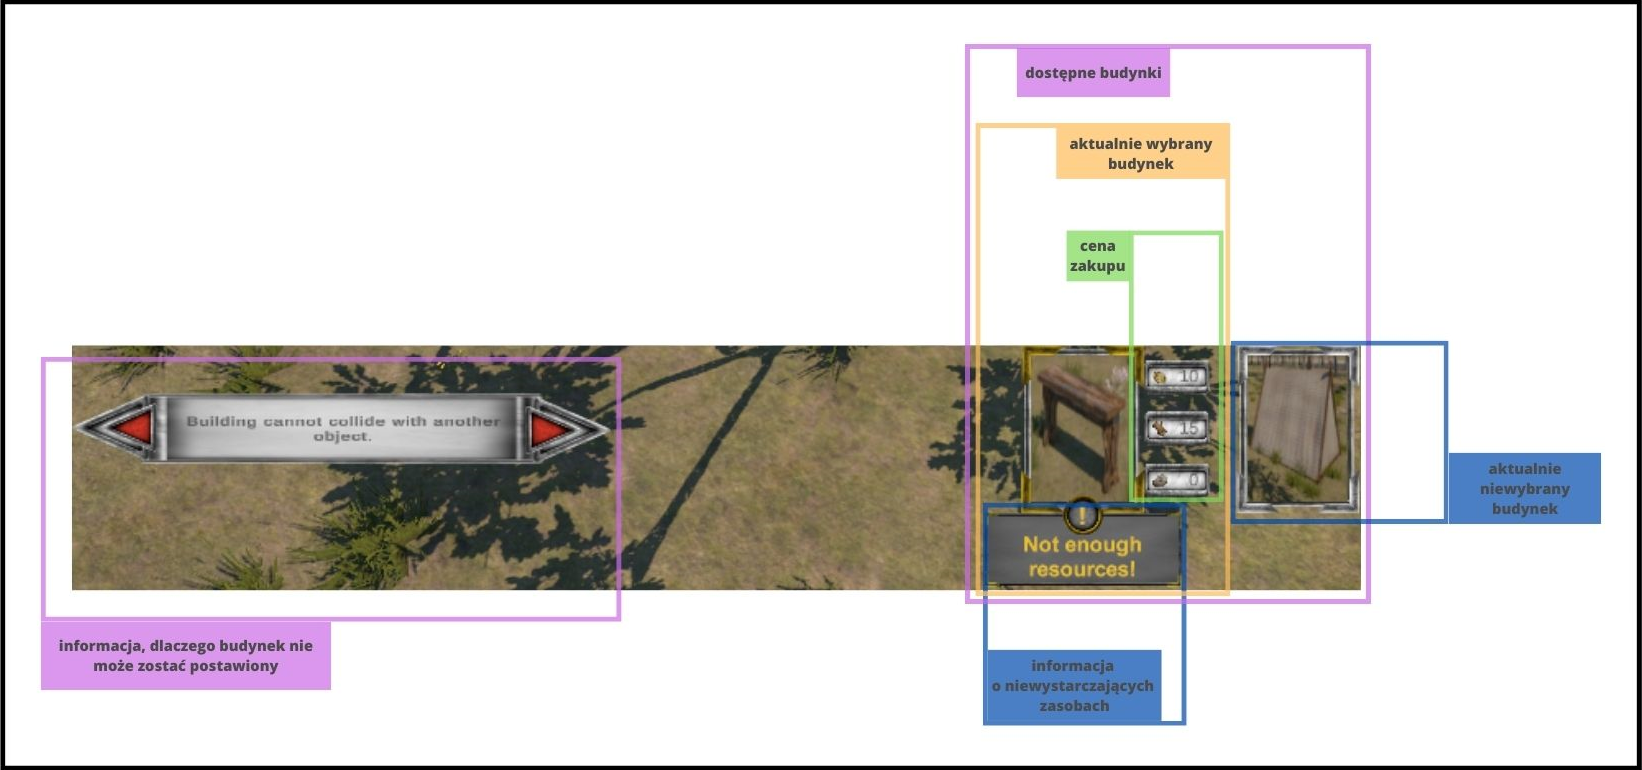
\includegraphics[width=0.9\textwidth]{images/ui/opis_ekementow_budowanie.png}
    \caption{Implementacja menu stawiania budynków, na którym pokazane są możliwe do zbudowania budowle 
    i szczegółowe informacje o ich dostępności.
    }\label{fig:compass}
\end{figure}

\subsection{Menu wydawania komend}
Gra umożliwia graczowi wykupienie usług najemników, jeśli dysponuje odpowiednimi funduszami. Gdy są oni już pod dowództwem użytkownika, może on im rozkazywać za pomocą 
menu wydawania komend. Po naciśnięciu klawisza "Q" pokazuje się lista dostępnych grup podwładnych, podzielonych według ich specjalizacji. Po wybraniu jednej z nich 
wylistowane zostaną możliwe do rozkazania czynności. W obu przypadkach gracz ma także możliwość anulowania. 
\begin{figure}[htbp]
    \centering
    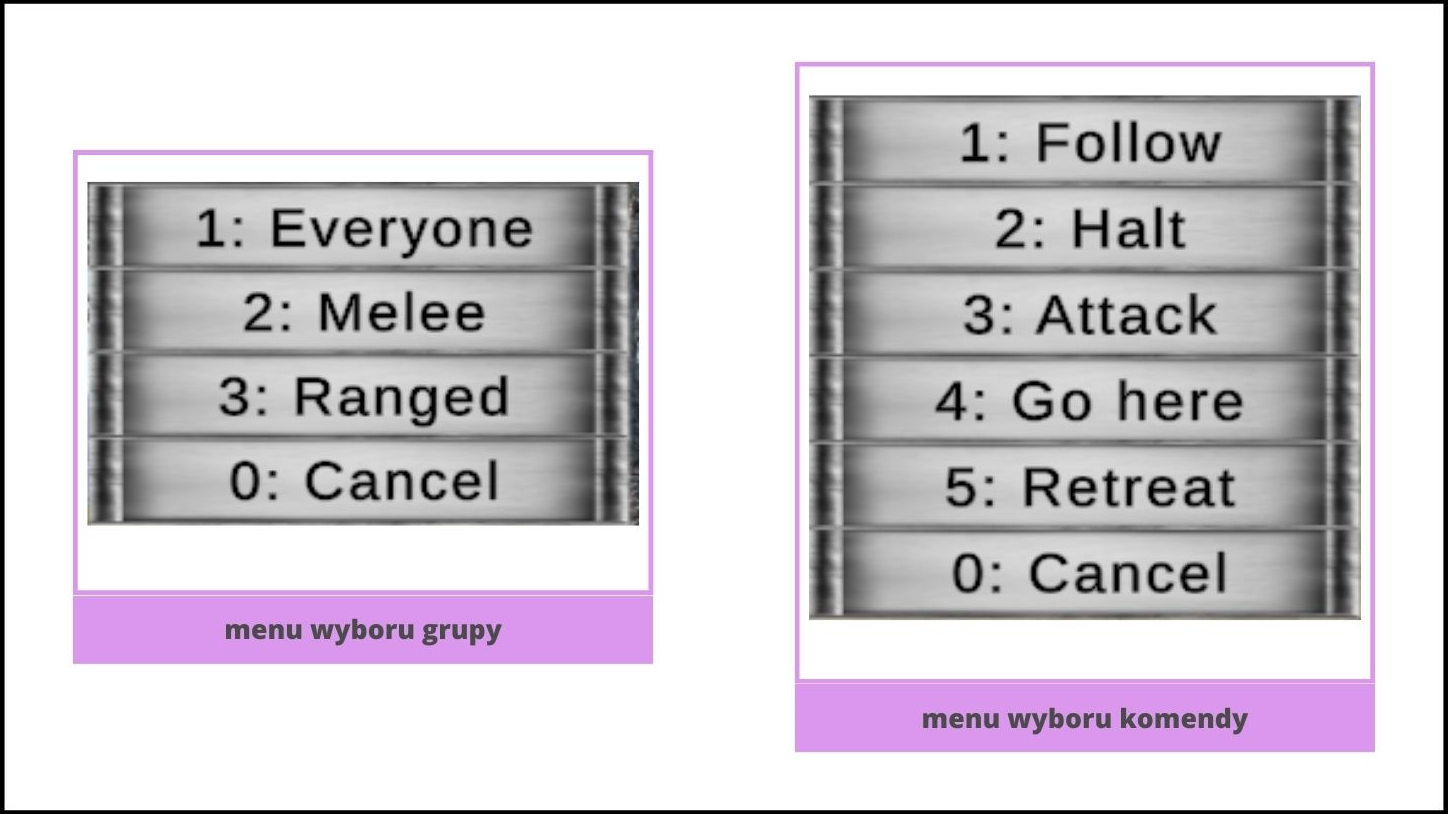
\includegraphics[width=0.9\textwidth]{images/ui/opis_ekementow_mwnu_wyboru_komendy.png}
    \caption{Implementacja menu wydawania komend.}\label{fig:cmd_menu}
\end{figure}

\subsection{Menu zapisu}
Po uznaniu przez gracza, że nie chce stracić aktualnego stanu gry, może go permamentnie zapisać w pamięci urządzenia, na którym włączony jest program. Po naciśnięciu 
klawisza "Z" pojawia sie menu zapisu. Gracz może odczytać z niego nazwę pliku, w którym zapisany zostanie stan gry. W menu znajduje się także informacja o tym, że 
poprzez ponowne naciśnięcie klawisza "Z" potwierdzi on zapis. 
\begin{figure}[htbp]
    \centering
    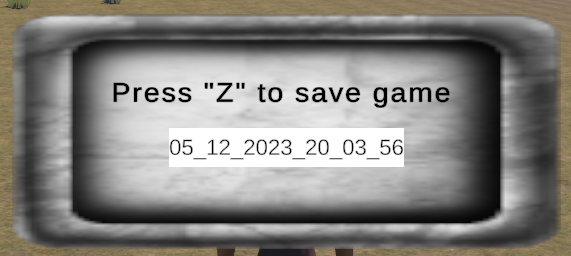
\includegraphics[width=0.9\textwidth]{images/ui/menu_zapisu.png}
    \caption{Implementacja menu zapisu.}\label{fig:men_zap}
\end{figure}

\subsection{Informacja o możliwej interakcji}
W świecie gry postać gracza nie jest odosobniona, co więcej może spotkać wiele różnorodnych osób, z którymi można porozmaiwać. Interaktywni
jednak nie są tylko ludzie, ale i surowce, które można zbierać. Jeśli możliwa jest interakcja,  wyświetlana jest informacja o takim stanie
 rzeczy. Zaraz pod kompasem pojawia się grafika instruująca, że po naciśnięciu klawisza "E" klawiatury, postać gracza wykona opisaną czynność.
 \begin{figure}[htbp]
    \centering
    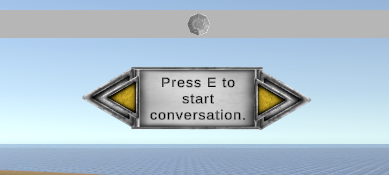
\includegraphics[width=0.9\textwidth]{images/ui/interakcja_rozmowa.png}
    \caption{Implementacja grafiki informującej o możliwości rozpoczęcia rozmowy.}\label{fig:rozmow}
\end{figure}
\begin{figure}[htbp]
    \centering
    \includegraphics[width=0.9\textwidth]{images/ui/interakcja_podnieś.png}
    \caption{Implementacja grafiki informującej o możliwości podniesienia przedmiotu.}\label{fig:przedmio}
\end{figure}

\subsection{Dziennik z zadaniami}
Niektóre postacie interaktywne mogą zlecić głównemu bohaterowi zadanie. Jeśli gracz się zgodzi, notatka o nim zostaje zapisana w dzienniku. Można do niego zajrzeć
wciskając klawisz "J". Graczowi ukaże się tytuł sygnalizujący główny cel zadania, streszczenie najważniejszych informacji oraz porada dotycząca mechanik gry np. 
"Wciśnij klawisz X, żeby stało się Y". To, że zadanie nie zostało jeszcze wykonane, sygnalizuje czerwony wykrzyknik w prawym, górnym rogu notatki. Gracz może 
zamknąć dziennik poprzez ponowne naciśnięcie klawisza "J".
\begin{figure}[htbp]
    \centering
    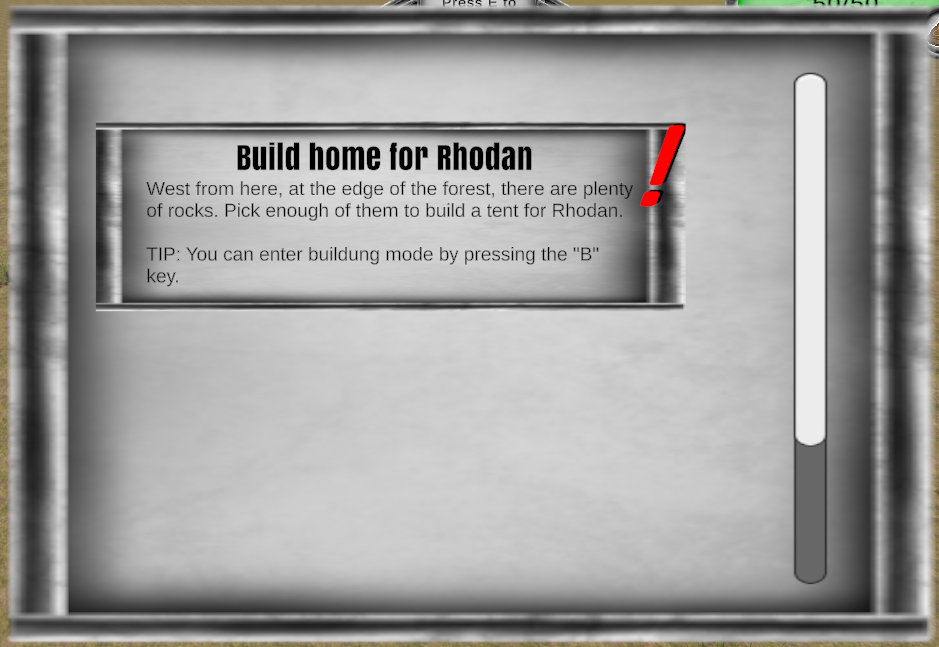
\includegraphics[width=0.9\textwidth]{images/ui/journal_quest.png}
    \caption{Implementacja dziennika z aktualnie zaczętym i nieukończonym zadaniem.}\label{fig:end_sc}
\end{figure}

\subsection{Ekran końca gry}
Postać gracza ma określoną liczbę punktów życia, które może stracić podczas potyczek z przeciwnikami. Gdy spadną one do zera gra kończy się, a główny bohater umiera.
W takim wypadku graczowi pojawia się ekran końca gry, który informuje go o śmierci oraz o możliwości przejścia do menu głównego. Aby jeszcze bardziej uwypuklić zakończenie 
rozgrywki, cały ekran zostaje przyciemniony.
\begin{figure}[htbp]
    \centering
    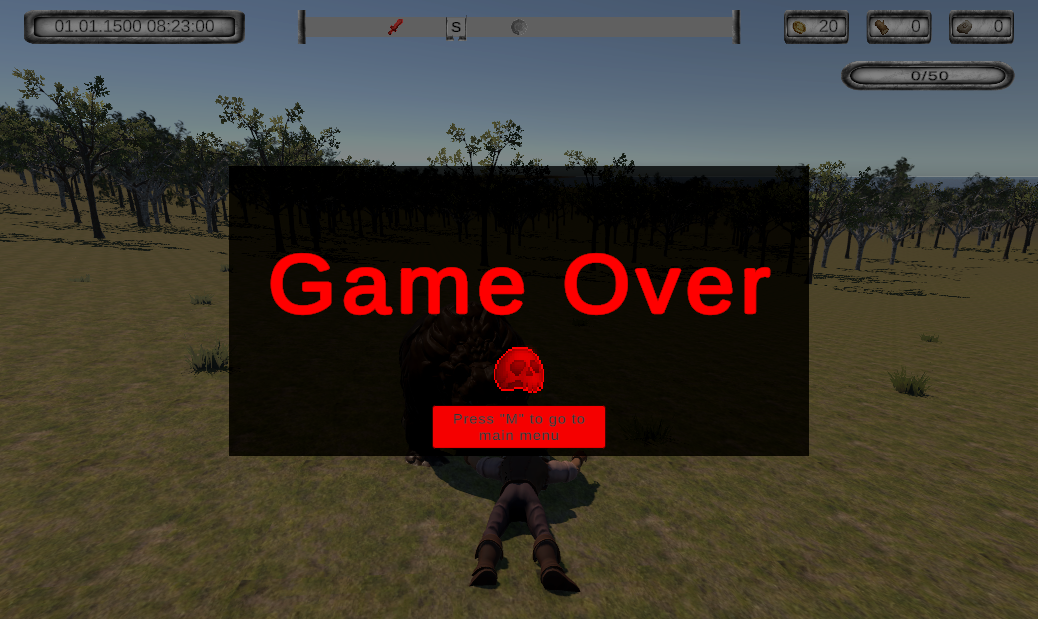
\includegraphics[width=0.9\textwidth]{images/ui/endgame_screen.png}
    \caption{Implementacja menu zapisu.}\label{fig:end_sc}
\end{figure}
\section{Menu główne (Zofia Sosińska)}\label{chap:menu_main}
Przed startem właściwej gry, użytkownikowi ukazuje się menu główne. Pełni ono funkcję reprezentatywną, więc ważne jest, aby współgrało ono z głównym programem.
Styl okna jest prosty i surowy, stawiając na skalę szarości przy doborze kolorów. Nawiązuje on do stylu interfejsu użytkownika występującego 
w później włączonym programie. Sprawia to, że gracz jeszcze przed zanurzeniem się w świat gry, ma jego przedsmak.

Zgodnie z projektem menu główne udostępnia trzy kluczowe funkcjonalności:
\begin{itemize}
    \item rozpoczęcie nowej gry;
    \item wczytanie zapisanej gry;
    \item wyjście z programu.
\end{itemize}

Przycisk nowej gry przenosi użytkownika do momentu startowego programu. Progres gry jest równy zeru, a wszystkie zadania dopiero czekają na wykonanie.

Po kliknięciu przycisku odczytu pojawia się lista zapisów, które w przeszłości użytkownik zdecydował się permanentnie przechować w pamięci urządzenia, na którym
włączony został program. Użytkownik może ją przeglądać ruszając suwakiem po prawej stronie. Po wybraniu jednej z opcji zostaje przeniesiony 
do świata gry o stanie takim, jaki został wczytany z pliku.

Ostatni przycisk udostępnia funkcjonalność wyjścia z gry. Po jego naciśnięciu użytkownik całkowicie wyłącza program.
\begin{figure}[htbp]
    \centering
    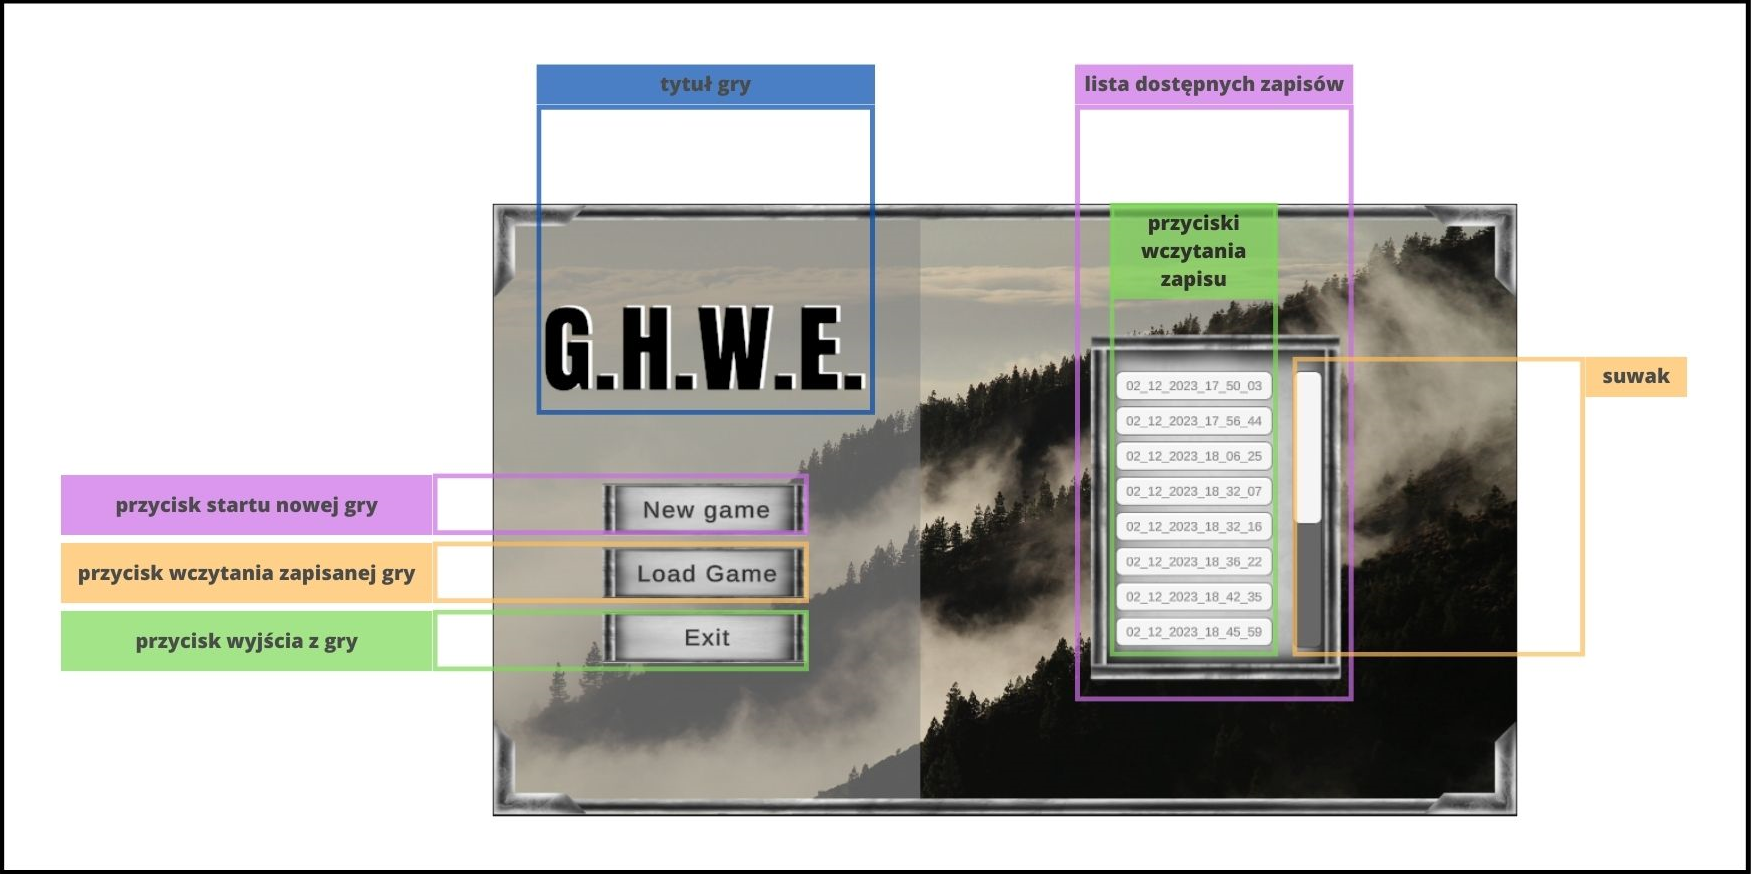
\includegraphics[width=0.9\textwidth]{images/ui/main_menu.png}
    \caption{Implementacja menu głównego.
    }\label{fig:compass}
\end{figure}


\section{Zasady działania kompasu (Zofia Sosińska)}\label{chap:naw_impl}

Projekt kompasu jest na tyle prosty, aby nie przytłoczyć gracza nadmierną liczbą bodźców. Składa się z horyzontalnego, jednolitego paska,
 na którym wyświetlane są najważniejsze informacje o otoczeniu, symbol ośmiokąta, wskazujący na przestrzeń znajdującą się centralnie przed bohaterem
  oraz z bocznych pasków, wyróżniających końce narzędzia.

\begin{figure}[htbp]
    \centering
    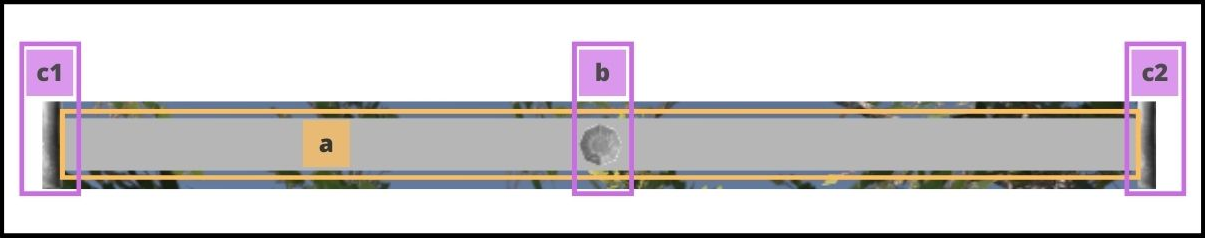
\includegraphics[width=0.9\textwidth]{images/ui/opis_ekementow_kompasu.png}
    \caption{Rozpiska elementów: a. główny pasek, b. symbol środka, c1., c2. paski końców kompasu.}\label{fig:compass_design}
\end{figure}
\FloatBarrier
Ikony wyświetlane na kompasie przedstawiają najważniejsze informacje w polu widzenia gracza, czyli stronę świata, w kierunku której jest on zwrócony, oraz przeciwników.
Poniżej przedstawiono kod odpowiedzialny za wyznaczenie pozycji symbolu na omawianym narzędziu. Wejściem jest komponent \texttt{RectTransform} symbolu przypisanego
danemu obiektowi oraz jego położenie. Po obliczeniu wektora prowadzącego do uzyskania np. pozycji wroga, wyznaczany jest kąt, o jaki musi się obrócić.
To jest przeliczane na pozycję na kompasie i jeśli obiekt znajduje się w polu widzenia postaci gracza to jest wyświetlany odpowiedni symbol.

\begin{figure}[htbp]
    \centering
    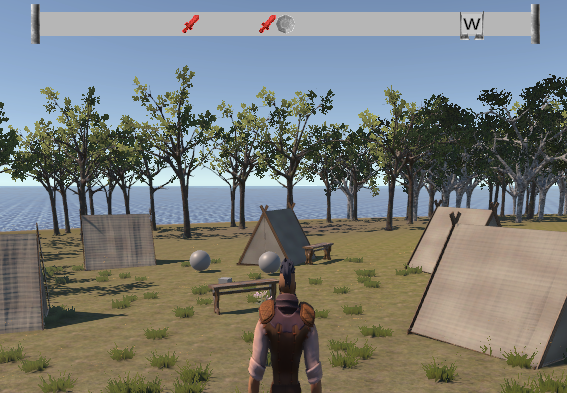
\includegraphics[width=0.9\textwidth]{images/ui/compass.png}
    \caption{Wizualizacja przypadku, w którym gracz patrzy centralnie na obozowisko wrogów. Na przeciwko oraz po lewej stronie znajdują się przeciwnicy, co jest zasygnalizowane na kompasie za pomocą symboli mieczy. Znajduje się na nim także informacja, że bohater jest lekko odchylony od Zachodu.
    }\label{fig:compass}
\end{figure}
\FloatBarrier
    \begin{lstlisting}[language=C++, caption=Fragment kodu odpowiedzialny za ustawienie symbolu na pasku kompasu.]
    void SetMarkerPosition(RectTransform markerTransform, Vector3 worldPosition)
    {
        Vector3 dirToTarget = worldPosition - CameraTransform.position;
        float angle = Vector2.SignedAngle(new Vector2(dirToTarget.x, dirToTarget.z), 
                                            new Vector2(CameraTransform.transform.forward.x, CameraTransform.transform.forward.z));
        float compassPositionX = Mathf.Clamp(
                                            2 * angle / Camera.main.fieldOfView, -1, 1);
        if (compassPositionX == 1 || compassPositionX == (-1))
        {
            markerTransform.anchoredPosition = new Vector2(0, 100);
        }
        else
        {
            markerTransform.anchoredPosition = new Vector2(
                compassBarTransform.rect.width / 2 * compassPositionX, 0);
        }
    }
    \end{lstlisting}
\FloatBarrier
Problem lokalizacji stron świata pojawił się, gdy nieprawidłowo wyświetlały się symbole po użyciu najprostszego rozwiązania. Na przykład dla Północy było to
pobranie wartości od \texttt{Vector3.forward}, co jest skrótowym zapisem \texttt{Vector3(0, 0, 1)}. Lewy dolny róg mapy jest położony w punkcie (0, 0, 0), co oznacza, że wymagane
jest przesunięcie, aby prawidłowo zasymulować strony świata. Północ i Południe  zostały przesunięte do połowy szerokości, a Wschód i Zachód - długości mapy. Każde z nich
zostało oddalone o 60000 jednostek, co pozwala na wiarygodną symulację stron świata na kompasie.

\begin{figure}[htbp]
    \centering
    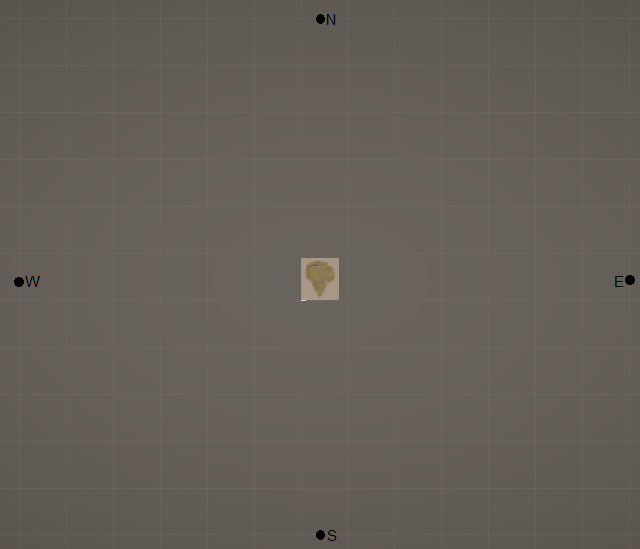
\includegraphics[width=0.9\textwidth]{images/ui/strony_swiata.png}
    \caption{Rozmieszczenie zasymulowanych stron świata.}\label{fig:world_sides}
\end{figure}
\FloatBarrier
Wykrycie wrogich jednostek znajduje się w funkcji Start. Każdemu obiektowi jest przypisywany symbol czerwonego miecza i w zależności od położenia wroga, obrazek wyświetlany jest odpowiednio na kompasie.
\begin{lstlisting}[language=C++, caption=Fragment kodu odpowiedzialny za połączenie wrogich obiektów na mapie z symbolami wyświetlonymi na kompasie.]
    void SetPositionOfEnemies()
    {
        foreach (
            var e in enemiesOnMap.Zip(enemiesOnUI, (x, y) => new {enemyOnMap = x, 
                                                                    enemyOnUI = y }))
        {
            SetMarkerPosition(e.enemyOnUI.GetComponent<RectTransform>(), 
                                e.enemyOnMap.transform.position);
        }
    }
\end{lstlisting}

\section{Mechanizm budowania (Bogna Lew)}\label{s:bud_impl}

Opracowany mechanizm umożliwia graczowi na przełączenie się w tryb budowania poprzez naciśnięcie klawisza \texttt{B}, który od razu
wyświetli podgląd bazowego obiektu. Widok budynku przemieszcza się przed postacią oraz odpowiednio obraca się razem z
nią. Efekt poruszania się podglądu został uzyskany za pomocą poniższego wzoru:
\begin{equation}
\begin{cases}
x = r \times sin(\alpha) \\
y = 0 \\
z = r \times cos(\alpha)
\end{cases}
\end{equation}

gdzie $x$, $y$ i $z$ to współrzędne odpowiednio względem osi X, Y i Z, $r$ to odległość środka obiektu od postaci
gracza, natomiast $\alpha$ to kąt o jaki jest on obrócony względem osi Y.

Podgląd budynku będzie widoczny do czasu, aż gracz go umieści naciskając prawy przycisk myszy bądź wychodząc z trybu
edycji naciskając klawisz \texttt{Escape}. Jeżeli widok budowli znajduje się w poprawnym do umieszczenia miejscu to jest on
podświetlany na zielono, w przeciwnym razie - na czerwono. Wybudowanie powoduje przywrócenie bazowych kolorów obiektu
oraz włącza wykrywanie kolizji z nim, dzięki czemu budynek poprawnie oddziałuje z otaczającym go środowiskiem.

\begin{figure}[h!]
    \centering
    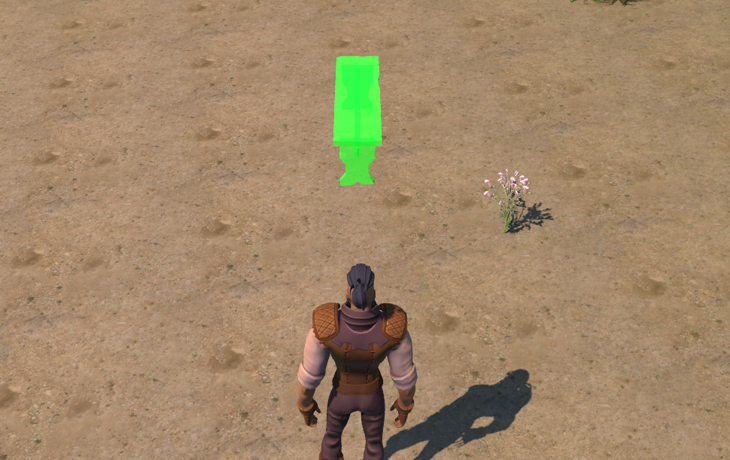
\includegraphics[width=1\textwidth]{images/implementacja/mechanizm_budowania/poprawne.png}
    \caption{Przykład podglądu w poprawnym umiejscowieniu.}
\end{figure}
\FloatBarrier

Do weryfikacji poprawności umiejscowienia budynku wykorzystano mechanizmy wyzwalacza (ang. \textit{trigger}) oraz rzucania
promienia (ang. \textit{raycasting}). Pierwszy z nich polega na wykrywaniu czy obiekt znalazł się w obszarze kolizji bez
brutalnego zatrzymywania go. Oznacza to, że może on przeniknąć przez inny element bez widocznych konsekwencji, jedynie
wysyłając sygnał, że dana sytuacja nastąpiła. Druga metoda natomiast polega na wypuszczeniu promienia o pewnej długości
w zadanym kierunku i sprawdzeniu, czy z czymś się zderzył.

Wyzwalacz został zastosowany do wykrywania kolizji z innymi obiektami na mapie, takimi jak postacie, czy elementy
scenerii niebędące terenem. W tym celu wykorzystano metody \verb|OnTriggerEnter()| i \verb|OnTriggerExit()|, które są wywoływane
odpowiednio gdy, dany obiekt znalazł się w obszarze kolizji innego elementu, bądź go opuścił. Każda z nich odpowiednio
zmienia poprzez zwiększenie bądź zmniejszenie wartości licznika kolizji obiektu. Jeżeli jego wartość jest różna od zera, tzn.
obiekt z czymś koliduje, to umiejscowienie jest uznawane za niepoprawne.

Drugi z mechanizmów został wykorzystany do sprawdzenia nachylenia podłoża. Efekt został osiągnięty poprzez rzucenie
promienia o niewielkiej długości z każdego z dolnych narożników obiektu i zliczeniu ile z nich wykryło kolizję z ziemią.
Brak wykrycia kolizji można zinterpretować jako zapadanie się bądź zbyt mocne lewitowanie danego narożnika nad
powierzchnią ziemi. Z tego powodu przyjęto, że jeśli co najmniej trzy z nich zderzyły się z podłożem, to umiejscowienie
jest poprawne.

\begin{figure}[h!]
    \centering
    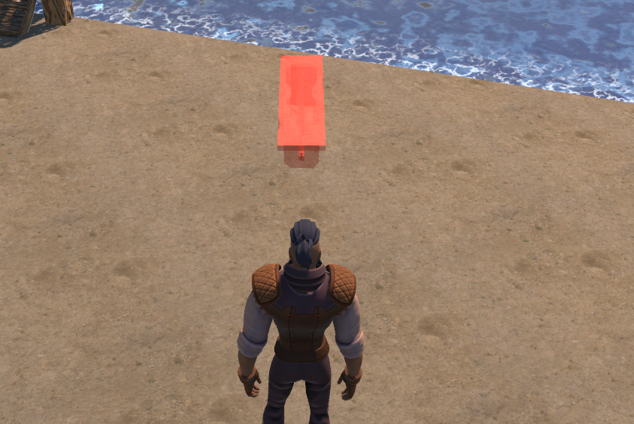
\includegraphics[width=1\textwidth]{images/implementacja/mechanizm_budowania/niepoprawne.png}
    \caption{Przykład podglądu w niepoprawnym umiejscowieniu.}
\end{figure}
\FloatBarrier

Dodatkowo metodę rzucania promienia wykorzystano do wykrycia kolizji z drzewami. Obiekty te są traktowane przez silnik
jako część terenu, przez co metoda wykorzystująca wyzwalacz pomija je. Dlatego w celu wykrywania kolizji z nimi
zdecydowano się na rzucenie dwóch grup promieni biegnących w głąb obiektu z naprzeciwległych krawędzi prostopadłych do
osi Y. Każdy z promieni biegnie w połowie wysokości obiektu i sięga przeciwnej ściany. Tak skomplikowany układ ma na
celu zapewnienie poprawności wykrywania kolizji w przypadku, gdy początki promieni znajdują się wewnątrz kolidującego
obiektu. Jeśli którykolwiek z nich zderzy się z drzewem, to wybrane miejsce jest uznawane za niepoprawne.

\begin{figure}[h!]
   \centering
   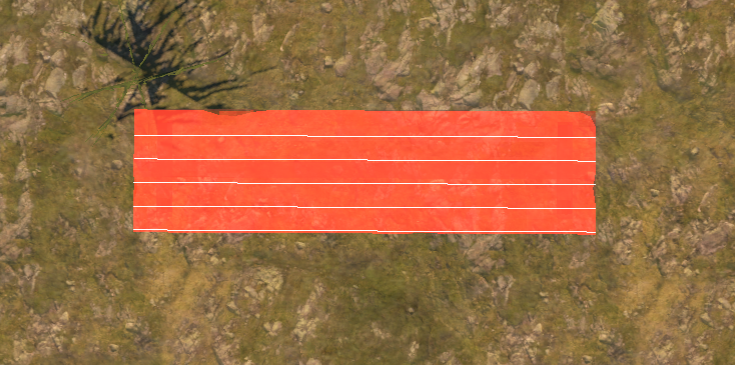
\includegraphics[width=1\textwidth]{images/implementacja/mechanizm_budowania/gizmos_drzewo_2.png}
   \caption{Widok z góry na siatkę promieni służących do wykrywania kolizji z drzewami.}
\end{figure}
\FloatBarrier
\begin{figure}[h!]
   \centering
   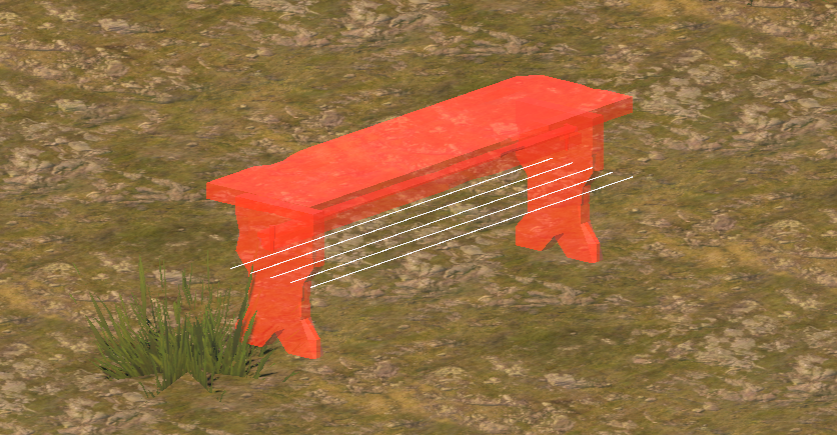
\includegraphics[width=1\textwidth]{images/implementacja/mechanizm_budowania/gizmos_drzewo_1.png}
   \caption{Widok z boku na siatkę promieni służących do wykrywania kolizji z drzewami.}
\end{figure}
\FloatBarrier

\section{System dialogów. Bartosz Strzelecki}

System dialogów jest podstawową metodą, którą gracz będzie wykorzystywał, aby pozyskać informacje  o świecie oraz celach misji.
Gracz może inicjować konwersacje z postaciami niezależnymi, po czym zostaną mu zaproponowane opcje sposobu prowadzenia rozmowy.
W zależności od wybranych opcji dialogowych gracz może się spodziewać różnych konsekwencji.


\begin{figure}[h]
\centering

\includegraphics[width=0.6\textwidth]{images/fallout3}
\caption{Kadr z gry Fallout 3 przedstawiający przykładowy dialog}
\end{figure}

\href{https://assetstore.unity.com/packages/tools/utilities/dialogue-editor-168329}{Dialogue Editor} autorstwa Grasshop Dev jest prostym narzędziem pozwalającym na szybkie dodawanie i modyfikację dialogów.
Zawiera zestaw elementów ułatwiających wdrożenie systemu do projektu oraz udostępnia struktury danych wykorzystywanych do tworzenia interfejsu użytkownika.
Podczas rozmowy z postaciami niezależnymi gracz będzie mógł pozyskać informację o geografii świata, możliwych zagrożeniach oraz zadaniach do wykonania. 
Podobne systemy występują w grach takich jak Pillars of Eternity oraz w grach z serii Mass Effect.


\section{Sztuczna inteligencja (Bartosz Strzelecki)}\label{s:ai_impl}
Nawigacja przeciwników została zrealizowana poprzez wbudowany w silnik Unity system \texttt{NavMesh}. Pozwala on na łatwe wyznaczenie powierzchni, po której mogą poruszać
się postacie niekontrolowane przez gracza oraz realizuje zadanie wyznaczania ścieżki dla tych postaci.

\begin{figure}[h]
\centering
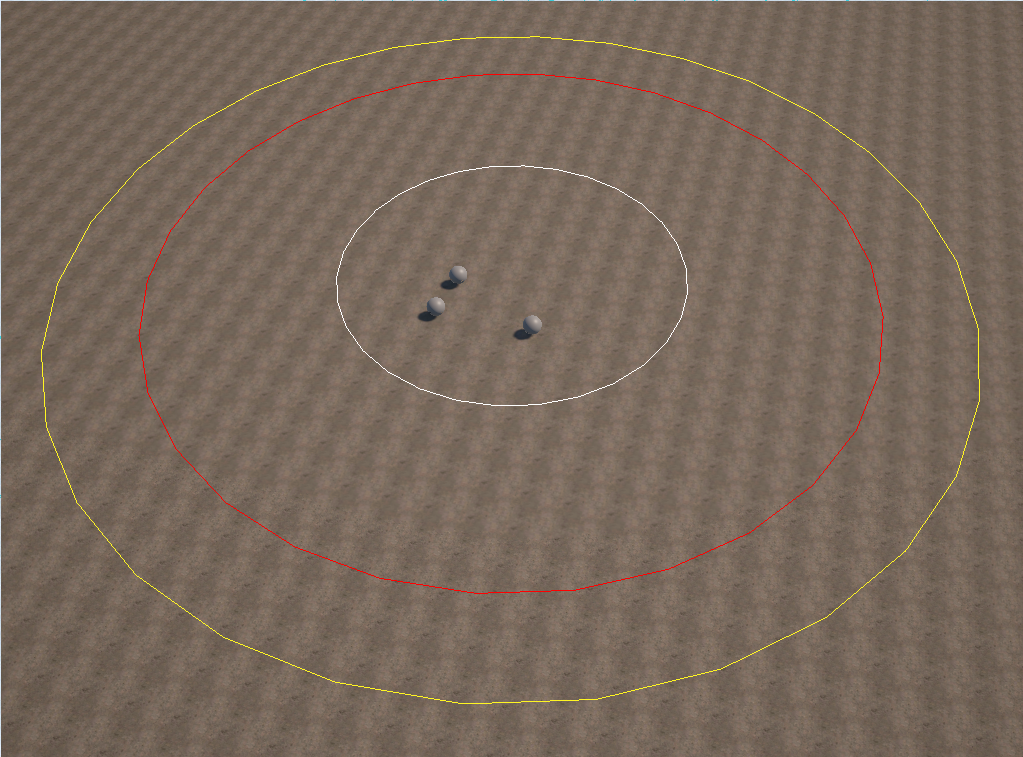
\includegraphics[width=0.9\textwidth]{images/ai}
\caption{Obraz przedstawia zasięgi odpowiednich regionów.}
\label{fig:regions}
\end{figure}
\FloatBarrier

Przeciwnicy są kontrolowani poprzez jeden obiekt przydzielający cele każdemu przypisanemu wrogowi. W normalnym trybie wrogowie poruszają się w sposób losowy
w obrębie wyznaczonej przestrzeni (biały okrąg na rys. \ref{fig:regions}). Kiedy przyjazne jednostki znajdą się w wystarczającej odległości (czerwony okrąg na rys. \ref{fig:regions}), przeciwnicy obiorą sobie za cel jedną z nich.
Po opuszczeniu przez drużynę gracza wyznaczonego obszaru (żółty okrąg na rys. \ref{fig:regions}) wrogowie wracają do poruszania się w sposób losowy w obrębie białego okręgu.


\begin{figure}[h]
\centering
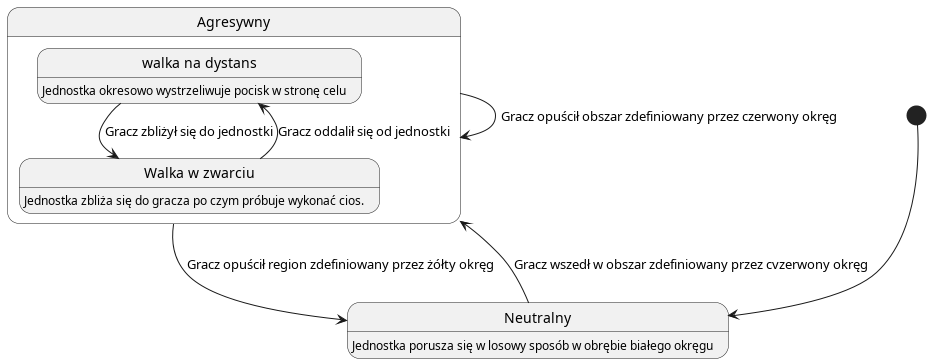
\includegraphics[width=1\textwidth]{uml/ai}
\caption{Diagram przedstawiający przepływ stanów dla sztucznej inteligencji przeciwników.}
\end{figure}
\FloatBarrier

\subsection{Mechanika zachowań klas jednostek}
\subsubsection{Jednostki walczące w zwarciu}
Zachowanie jednostek bliskiego zasięgu polega na wybraniu przeciwnika będącego w czerwonym obszarze (rys. \ref{fig:regions}), który ma najwyższą
wartość priorytetu obliczonego między innymi na podstawie odległości, ilości innych atakujących przeciwników oraz klasy celu.
Jednostka posiadająca cel ataku zmierza w jego kierunku, obierając najkrótszą drogę. Po dotarciu do celu podróży jednostki biorące udział w walce
losują naprzemiennie liczby, od których zależy wynik walki, jak i aktualnie wykorzystywana animacja.

\subsubsection{Jednostki walczące na dystans}
Takie jednostki wystrzeliwują w stronę przeciwników pociski, których celność jest reprezentowana przez dwie strefy (rys. \ref{fig:acc2}). Jedną oznaczającą 50\% celności,
czyli rozrzut, który będzie posiadała połowa pocisków, oraz drugą oznaczającą maksymalny rozrzut. Ten mechanizm pozwala na łatwe zamodelowanie
celności ze względu na odległość, wielkość celu oraz na osłony, za którymi może stać wroga jednostka.
\begin{figure}[h]
\centering
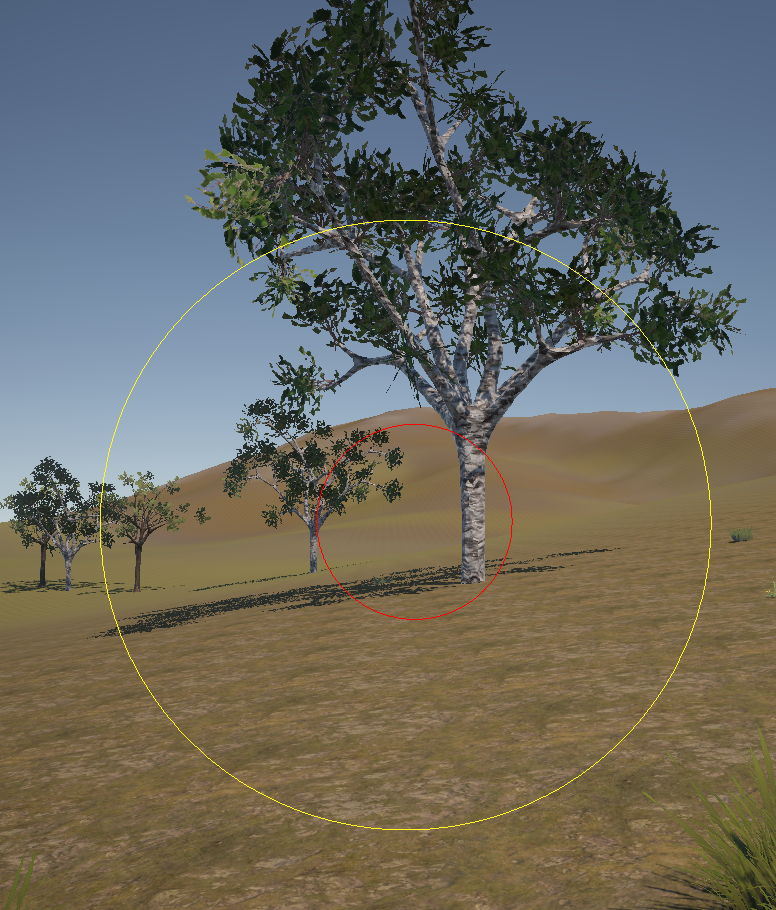
\includegraphics[width=0.6\textwidth]{images/acc}
\caption{Reprezentacja graficzna celowania widziana z perspektywy jednostki dalekozasięgowej. Czerwony okrąg reprezentuje obszar, w którym znajdzie się 50\% pocisków. Żółty obszar pokazuje maksymalny rozrzut.}
\label{fig:acc2}
\end{figure}
\subsubsection{Jednostki hybrydowe}
Obejmują zachowanie dwóch powyższych klas jednostek w zależności od odległości od przeciwnika.
W sytuacji, w której wroga jednostka znajduje się w pobliskim otoczeniu, wykorzystywany jest kod przeznaczony dla jednostek bliskiego zasięgu,
w przeciwnym przypadku wybierana jest logika jednostek zasięgowych.

\subsection{Sztuczna inteligencja przyjaznych jednostek.}

Kontrola jednostek przez gracza odbywa się za pomocą wybory jednej z opcji w dwóch fazach
\begin{itemize}
\item Faza wybrania jednostek
  \begin{itemize}
    \item wszyscy
    \item jednostki bliskozasięgowe 
    \item jednostki hybrydowe
    \item jednostki dalekozasięgowe
    \item opcja anulowania wyboru
  \end{itemize}

\item Faza wydania rozkazu
  \begin{itemize}
    \item podążanie za graczem
    \item zatrzymanie
    \item atak
    \item podejście do wskazanego przez gracza miejsca
    \item ucieczka
    \item opcja anulowania rozkazu
  \end{itemize}
\end{itemize}

Wydanie rozkazu polega na kliknięciu przycisku odpowiedzialnego za wejście w tryb wydawania poleceń, a następnie
wybraniu numeru opcji reprezentującej grupę jednostek, której komenda ma dotyczyć. Ostatecznie należy podać numer rozkazu, który zostanie wydany.
Przykładowa reprezentacja graficzna systemu jest widoczna na rysunku \ref{fig:mnb}.
Wykorzystanie tego modelu pozwala na łatwe rozwinięcie systemu o dodanie nowych metod wyboru grup jednostek oraz możliwych instrukcji dla przyjaznych agentów.

\begin{figure}[h]
\centering
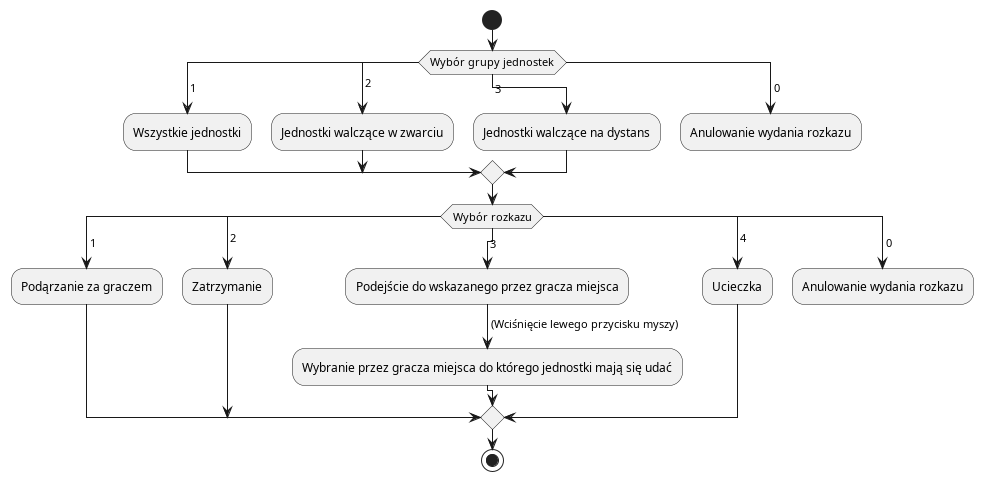
\includegraphics[width=1\textwidth]{uml/commands}
\caption{Wizualizacja przepływu sterowania podczas wydawania poleceń jednostkom.}
\end{figure}

\section{Widzenie przez horyzont (Bartosz Strzelecki)}\label{s:wid_impl}
Efekt został osiągnięty poprzez zmodyfikowanie potoku renderowania w taki sposób, że w zależności od wartości w buforze głębi jest wykorzystywany inny shader.
W tym przypadku, jeżeli sfera jest przysłonięta przez ścianę, jest ona narysowana, a w przeciwnym wypadku jest uruchamiany pusty shader.
"Unity domyślnie sortuje obiekty na podstawie odległości od kamery. Tak więc
w miarę zbliżania się obiektu do kamery, będzie on rysowany nad wszystkimi obiektami znajdującymi się dalej od kamery.
W większości przypadków sprawdza się to dobrze podczas tworzenia gier, ale
znajdą się sytuacje, w których będziemy chcieli mieć większą kontrolę nad sortowaniem obiektów na scenie. Używając bloku \verb|Tags\{\}| możemy kontrolować to sortowanie.
Unity udostępniło nam kilka domyślnych kolejek renderowania, z których każda ma unikalną wartość, którą
kieruje Unity, kiedy należy narysować obiekt na ekranie. Te wbudowane kolejki renderowania
nazywają się \verb|Background|, \verb|Geometry|, \verb|AlphaTest|, \verb|Transparent| i \verb|Overlay|." \cite{shaderscookbook}. Wykorzystując ten mechanizm
możliwe jest uzyskanie efektu widzenia przez postać gracza poprzez horyzont. Uzyskujemy przez to efekt podobny do tego zaimplementowanego w grze \textit{Dead by Daylight} (por. \ref{chap:dbd}).

Po naciśnięciu przycisku \texttt{E} następuje zagranie animacji opisanej wzorami

\begin{equation}
w(t, offset) = 1.1 \times 2.1^{-\left(\frac{{\left(\sin(t) + 1 - 0.4 - \text{{offset}}\right)^2}}{{0.02}}\right)}
\end{equation}

oraz

\begin{equation}
w(t, 0) - w(t, -0.2) + w(t, -1) - w(t, -1.2)
\end{equation}

Od podanych funkcji zależy przeźroczystość, jak i natężenie efektu Fresnela. 

\begin{figure}[h]
    \centering
    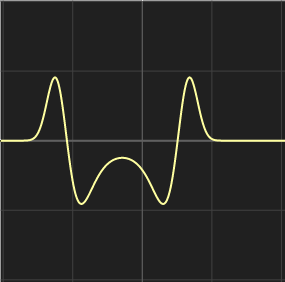
\includegraphics[width=0.5\textwidth]{images/g}
    \caption{Wykres przedstawiający funkcję opisującą natężenie efektu w animacji markera.}
\end{figure}



\begin{lstlisting}[language=C++, caption=Fragment shadera odpowiedzialny za animację.]
fixed4 frag (v2f i) : SV_Target
{
  float t =  6.2 * _Progress - 0.6;
  fixed4 pattern = tex2D(_PatternTex, i.uv + _Speed *t);
  float fresnelInfluence = dot(i.worldPos, i.viewDir);
  float saturatedFresnel = saturate(1 - fresnelInfluence);

  float g = w(t, 0) - w(t, -0.2) + w(t, -1) - w(t, -1.2);
  float4 color = pow(saturatedFresnel, g * _FresnelPow) * (_Color * _ColorIntensity) * pattern;
  color.a *= dot(i.worldPos, i.viewDir);
  return color;
}
\end{lstlisting}

\begin{figure}[h]
\centering
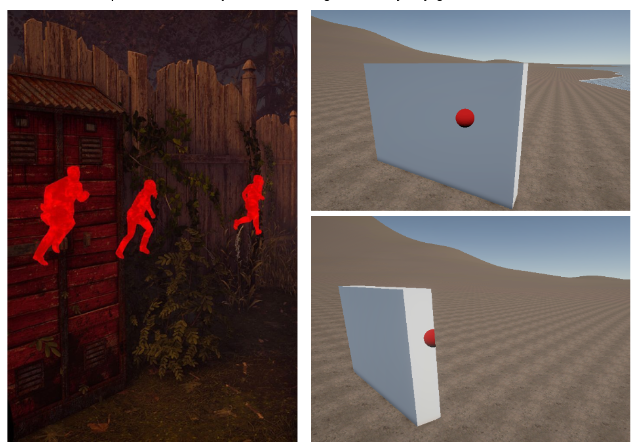
\includegraphics[width=0.6\textwidth]{images/shader}
\caption{Zachowanie programu cieniującego w przypadku przysłaniania markera przez przeszkody.}
\end{figure}

\section{Zapis i odczyt stanu gry (Bartosz Strzelecki)}\label{s:save_impl}

Gracz w dowolnym momencie rozgrywki może przerwać grę i dokonać zapisu. Wykonuje to
za pomocą skrótu klawiszowego F8. Powoduje to zapisanie na dysk danych wszystkich obiektów posiadających
komponent "Saveable". Strukturę serlializowanych danych reprezentuje plik proto \ref{proto}.
\lstinputlisting[caption=Plik .proto reprezentujący strukturę zapisu stanu gry, label=proto]{images/game_save.proto}

Powstały po zapisie plik jest przechowywany na dysku w lokalizacji zdefiniowanej przez stałą \verb|Environment.SpecialFolder.MyDocuments| w formie binarnej (rys. \ref{save}).
W tym przypadku zapamiętywane są jedynie dane, które zmieniają się w trakcie rozgrywki, takie jak położenie gracza, przeciwników, itd. 
Zawartość statyczna taka jak krzywizna terenu i flora występująca na mapie nie jest zapisywana, a jej wczytywanie jest rozwiązywane
w trackie ładowania sceny przez Unity Runtime.

\begin{figure}[h]
\centering
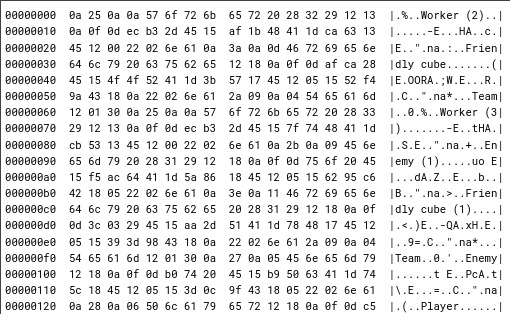
\includegraphics[width=1\textwidth]{images/save}
\caption{Zawartość przykładowego zapisu gry.}
\label{save}
\end{figure}

W momencie, w którym gracz zażąda odczytania zapisu gry, następuje proces odwrotny. Odpowiednie obiekty zostają utworzone,
a następnie przypisywane są im wartości na podstawie danych zawartych w pliku zapisu. Obiekty identyfikowane
są po ich nazwie, w taki sposób, w jaki są zarządzane przez Unity.
Tę akcję gracz wykonuję za pomocą przycisku F9 lub poprzez wybranie interesującego go zapisu z menu głównego.


\section{Przebieg rozgrywki}
Gracz zaraz po rozpoczęciu rozgrywki znajduje się w małej wiosce. Pierwszym
elementem przyciągającym uwagę gracza, jest postać o imieniu Amargein, która oferuje
nagrodę za pokonanie groźnego niedźwiedzia buszującego w pobliskim lesie. Użytkownik jednak
szybko się orientuje, że nie jest w stanie pokonać bestii w pojedynkę.

Po głębszych poszukiwaniach gracz znajduję dwójkę najemników, którzy byliby w stanie
wesprzeć główną postać za odpowiednią opłatą. Początkowo użytkownik nie może sobie
pozwolić na takie wydatki i jest zmuszony do znalezienia prostszego zadania
w celu zadbania o odpowiedni stan finansów.

[...]

Po wykonaniu uprzedniego zadania gracz jest już w stanie wykupić pomoc dwóch okolicznych
najemników. Po rozmowie każdy z nich jest gotów zgodzić się na opłatę w wysokości 10 złotych monet.
Tak przygotowana drużyna gracza jest gotowa na wyruszenie na przygodę, by uratować
mieszkańców wioski od niedźwiedzia terroryzującego osadę.

Gracz, wykorzystując swoje zdolności nawigacji, udaje się na wschód i po krótkim czasie jest w stanie zidentyfikować zagrożenie.
Widząc swój cel, gracz wydaje rozkaz ataku. Wynajęte jednostki szybko uporały się z niedźwiedziem, wykorzystując zarówno
broń białą, jak i łuk.

Po powrocie do wioski gracz jest uznany za bohatera, który ocalił wszystkich mieszkańców i zostaje odpowiednio nagrodzony.


